\documentclass[crop,tikz]{standalone}

\usepackage[utf8]{inputenc}
\usepackage{ifthen}
\usepackage{amsmath}
\usepackage{amssymb}

\newcommand{\reals}{\mathbb{R}}

% 'crop' is the default for v1.0, before it was 'preview'
%\usetikzlibrary{...}% tikz package already loaded by 'tikz' option


\begin{document}

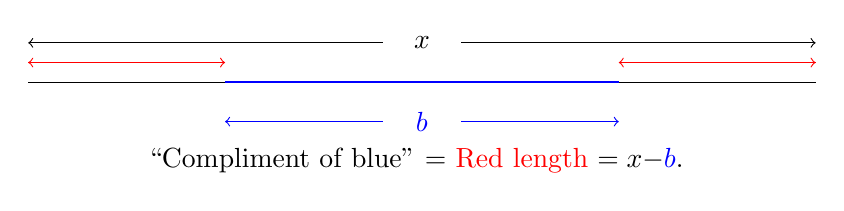
\begin{tikzpicture}

	%draw the real line
	\draw[black] (0,0) -- (10,0);
	\draw[black, ->] (5-0.5,0.5) -- (0,0.5);
	\draw[black, ->] (5+0.5,0.5) -- (10,0.5);
	\node[align=center] at (5,0.5) {$x$};
	\draw[blue, thick] (2.5,0) -- (7.5,0);
	\draw[blue, ->] (5-0.5,-0.5) -- (2.5,-0.5);
	\draw[blue, ->] (5+0.5,-0.5) -- (7.5,-0.5);
	\node[blue, align=center] at (5,-0.5) {$b$};
	\draw[red, ->] (0,0.25) -- (2.5,0.25);
	\draw[red, ->] (2.5,0.25) -- (0,0.25);
	\draw[red, ->] (7.5,0.25) -- (10,0.25);
	\draw[red, ->] (10,0.25) -- (7.5,0.25);
	
	\node[align=center] at (5,-1) {``Compliment of blue" $=$ \textcolor{red}{Red length} $= x-$\textcolor{blue}{$b$}. };
	
\end{tikzpicture}

\end{document}